\section{\tl{Application of FAMD to the dataset}}
\en{Another method for dimensionality reduction is Factor Analysis of Mixed Data. FAMD combines both views, and creates a set of transformed components that contain information from both sets of variables.
}
\subsection{\en{Without scaling or balancing:}}
\en{
\begin{figure}[H]
    \centering
    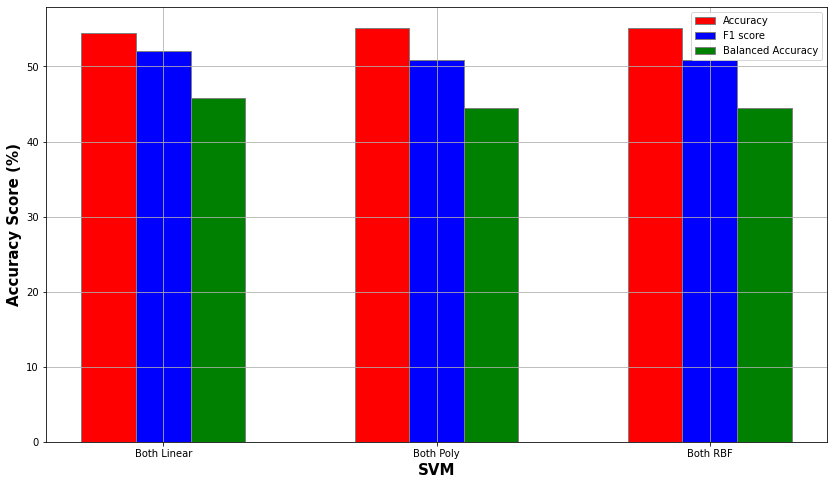
\includegraphics[width=\textwidth]{figures/Results/FAMD/FAMD_out.png}
    \caption[\en{FAMD SVM Classification metrics}]{\en{Classification metric using both views (imaging and genetic) on the SVM kernels previously mentioned (Linear, Polynomial, RBF), using the FAMD transformed imaging and genetic data.}}
\end{figure}

% \begin{figure}[H]
%     \centering
%     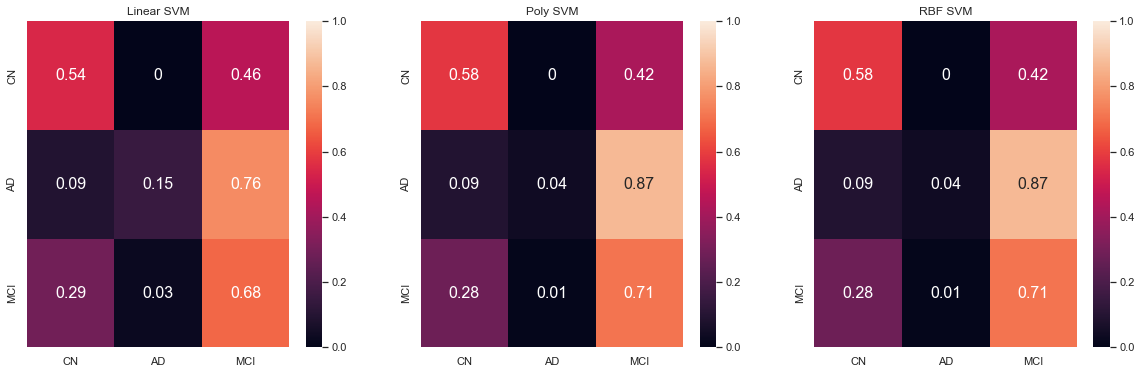
\includegraphics[width=\textwidth]{figures/Results/FAMD/FAMD_CM_out.png}
%     \caption[\en{FAMD SVM Confusion Matrices}]{\en{The Confusion Matrices for each class, per SVM kernel, for the FAMD transformed imaging and genetic data.}}
% \end{figure}

\begin{figure}[H]
    \centering
    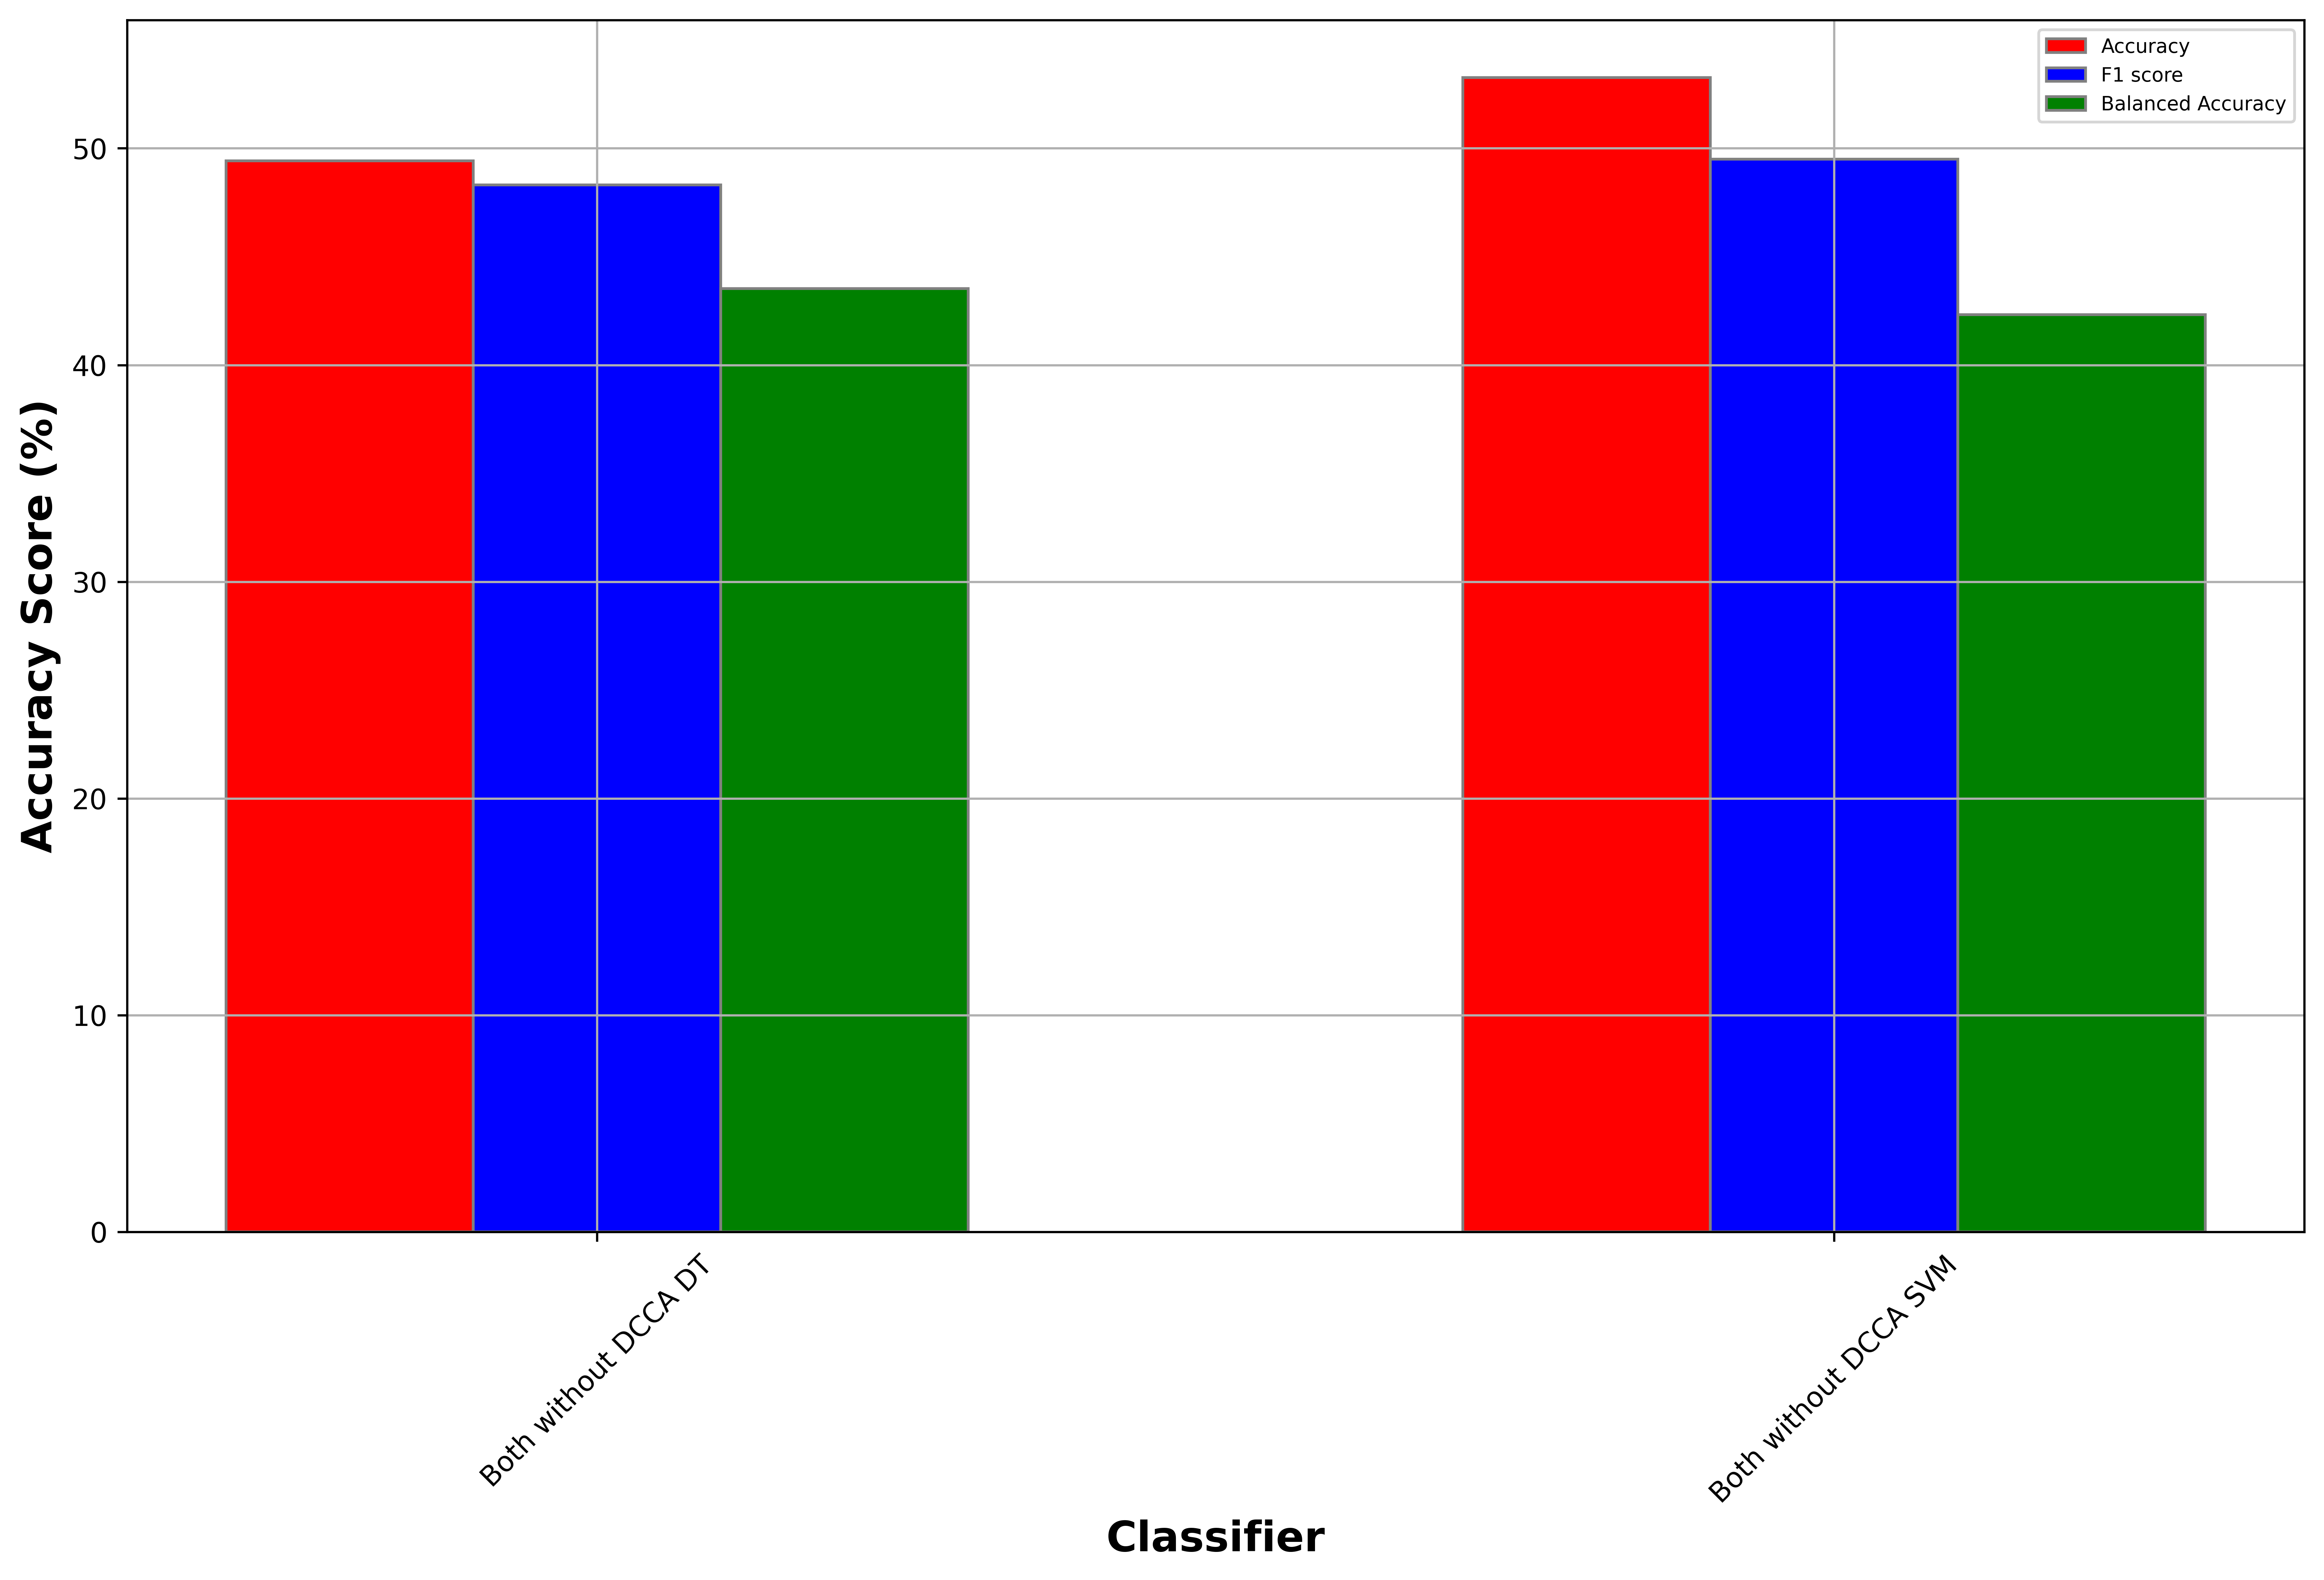
\includegraphics[width=\textwidth]{figures/Results/FAMD/Bagging_FAMD_out.png}
    \caption[\en{FAMD Bagging Classification metrics}]{\en{Classification metric using Bagging on the FAMD transformed imaging and genetic data.}}
\end{figure}

% \begin{figure}[H]
%     \centering
%     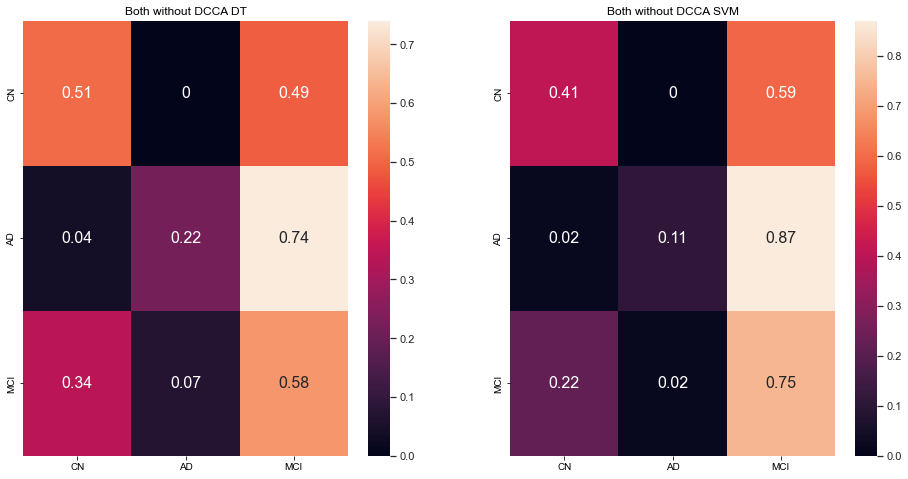
\includegraphics[width=\textwidth]{figures/Results/FAMD/Bagging_FAMD_CM_out.png}
%     \caption[\en{FAMD Bagging Confusion Matrices}]{\en{The Confusion Matrices for each class, with Bagging, for the FAMD transformed imaging and genetic data.}}
% \end{figure}

\begin{figure}[H]
    \centering
    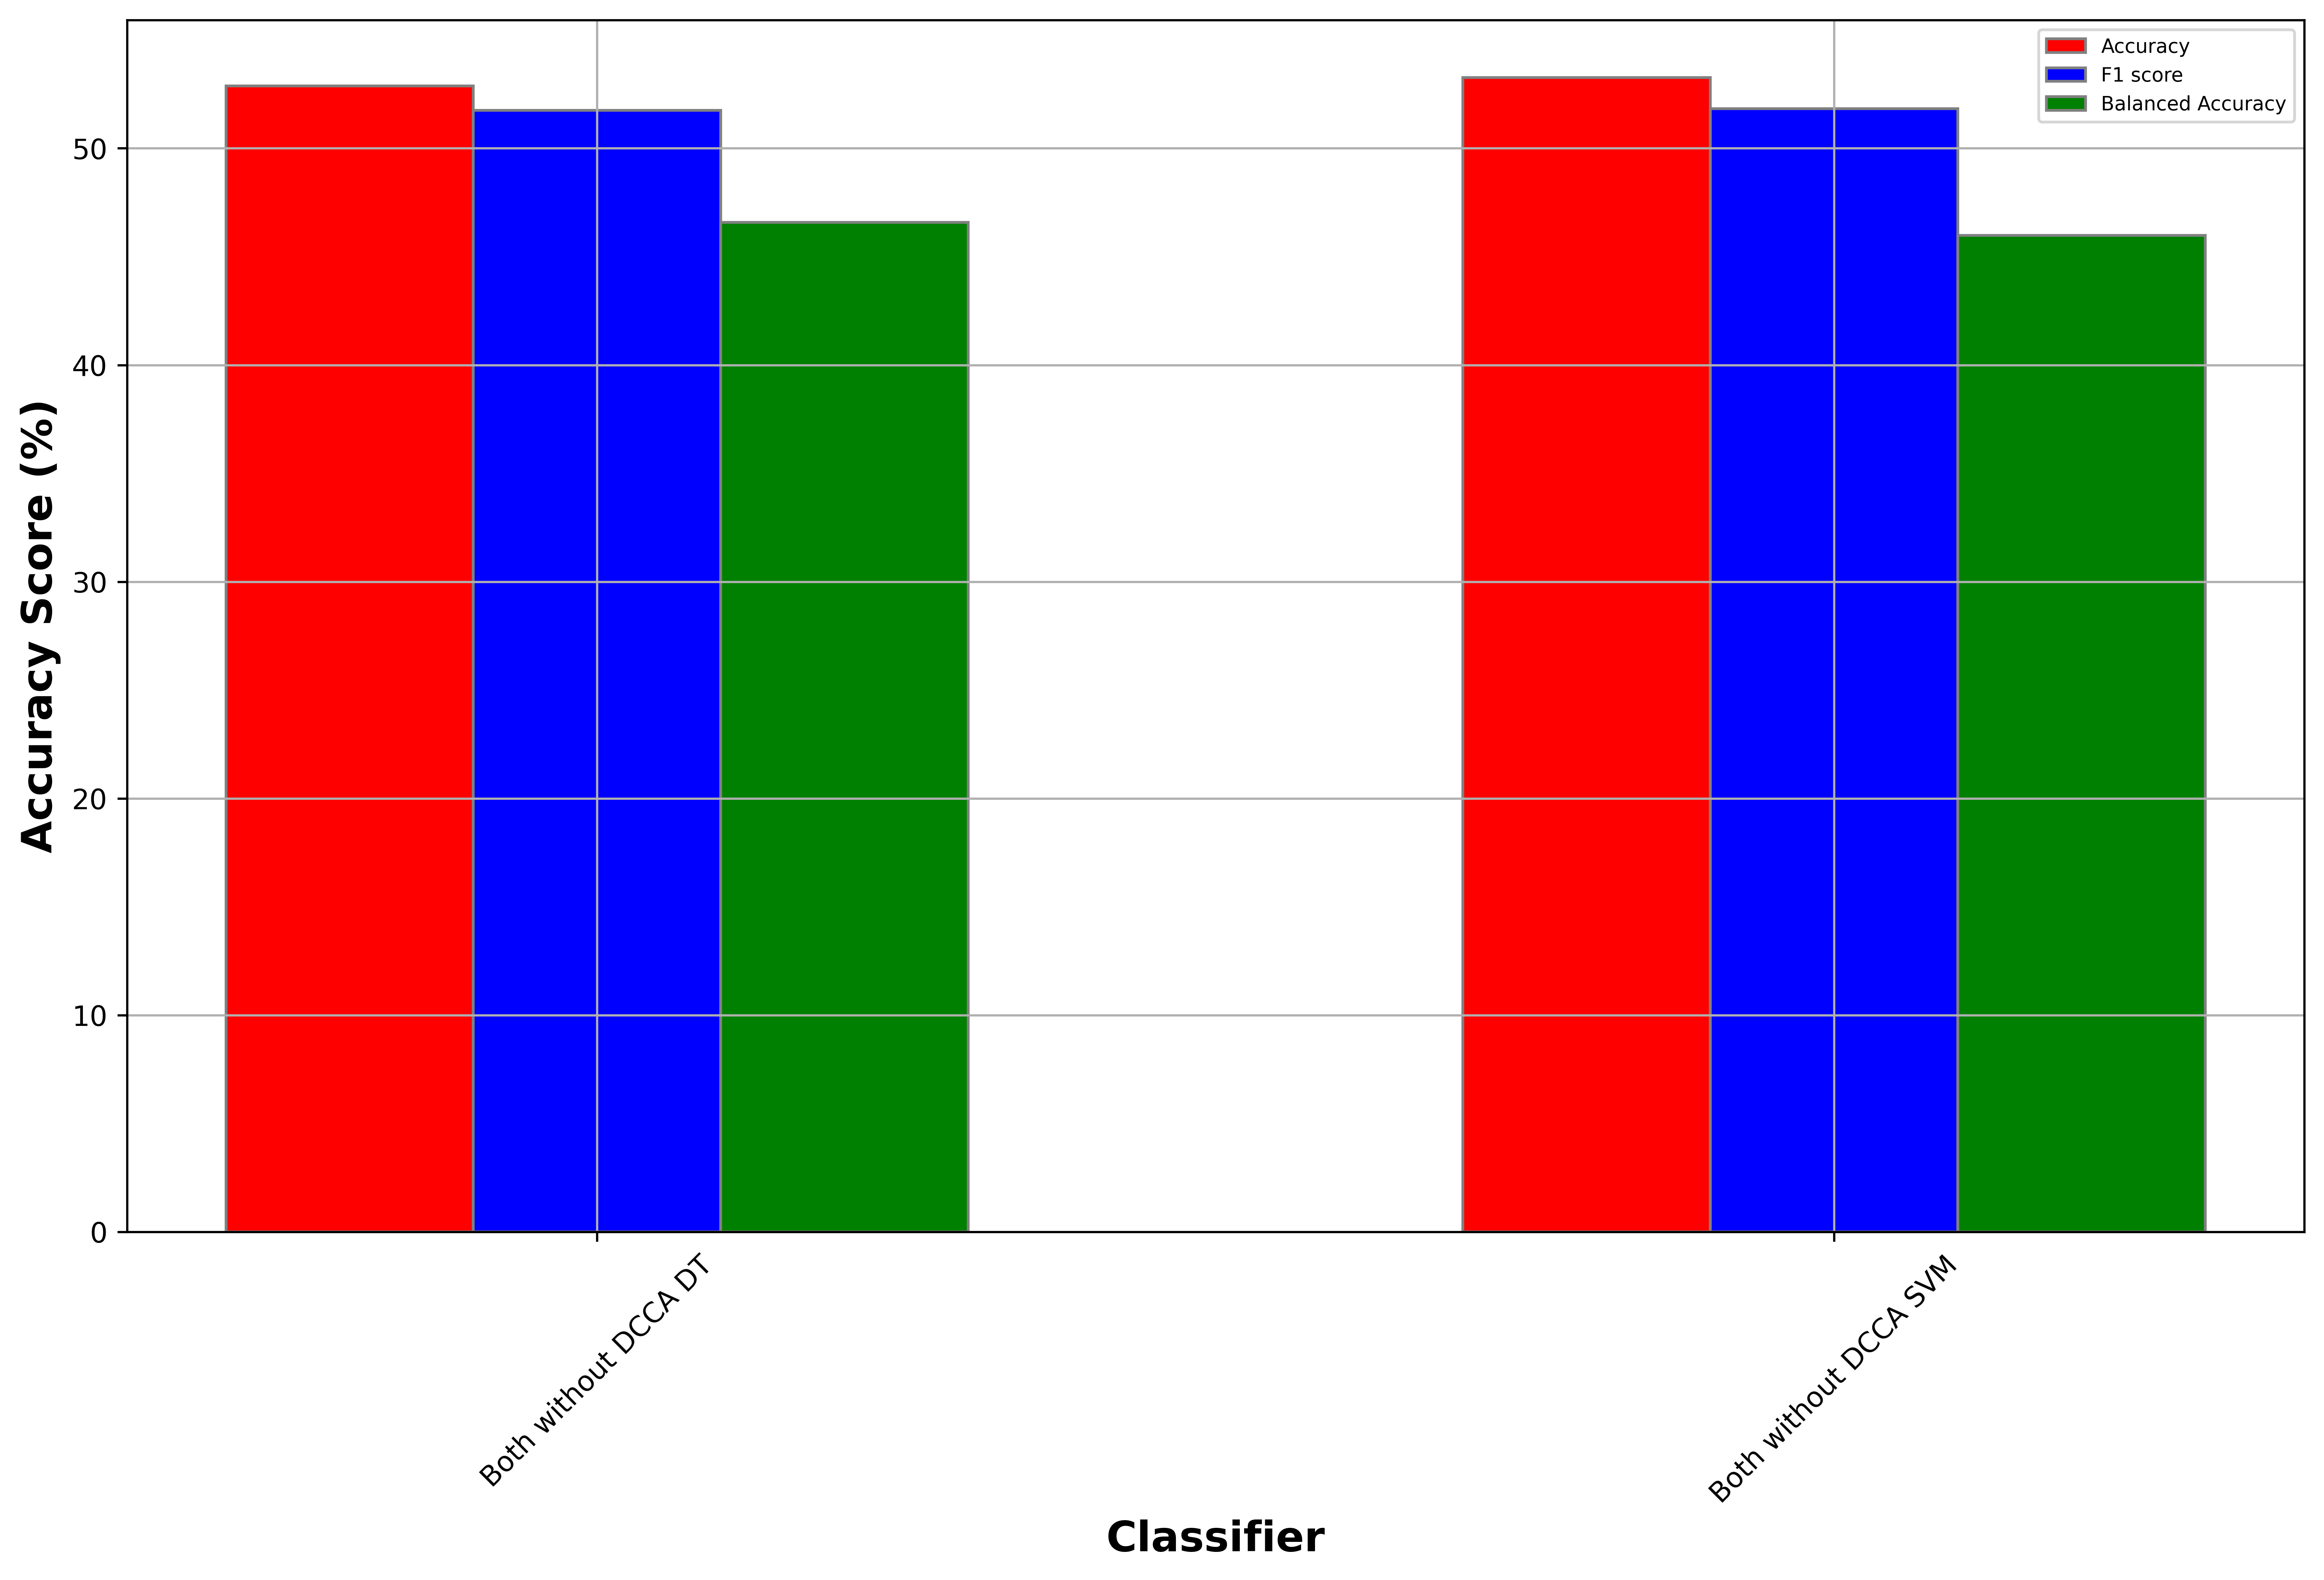
\includegraphics[width=\textwidth]{figures/Results/FAMD/AdaBoost_FAMD_out.png}
    \caption[\en{FAMD AdaBoost Classification metrics}]{\en{Classification metric using AdaBoost on the FAMD transformed imaging and genetic data.}}
\end{figure}

% \begin{figure}[H]
%     \centering
%     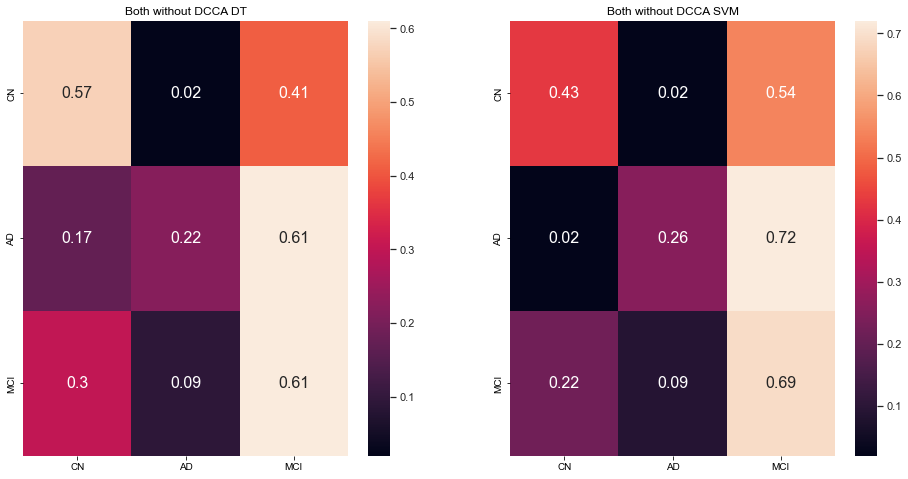
\includegraphics[width=\textwidth]{figures/Results/FAMD/AdaBoost_FAMD_CM_out.png}
%     \caption[\en{FAMD AdaBoost Confusion Matrices}]{\en{The Confusion Matrices for each class, with AdaBoost, for the FAMD transformed imaging and genetic data.}}
% \end{figure}

}
\subsection{\en{With scaling and balancing:}}
\en{
\begin{figure}[H]
    \centering
    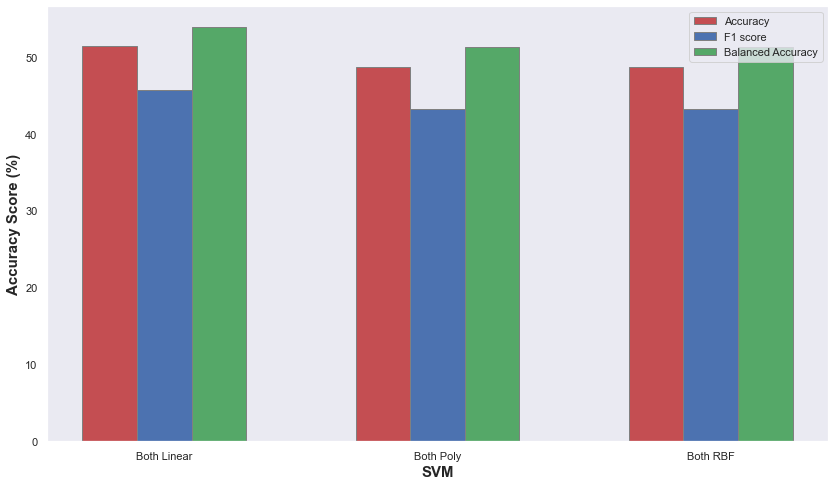
\includegraphics[width=\textwidth]{figures/Results/FAMD/FAMD_with.png}
    \caption[\en{FAMD SVM Classification metrics with scaling and balancing}]{\en{Classification metric using both views (imaging and genetic) on the SVM kernels previously mentioned (Linear, Polynomial, RBF), using the FAMD transformed imaging and genetic data.}}
\end{figure}

% \begin{figure}[H]
%     \centering
%     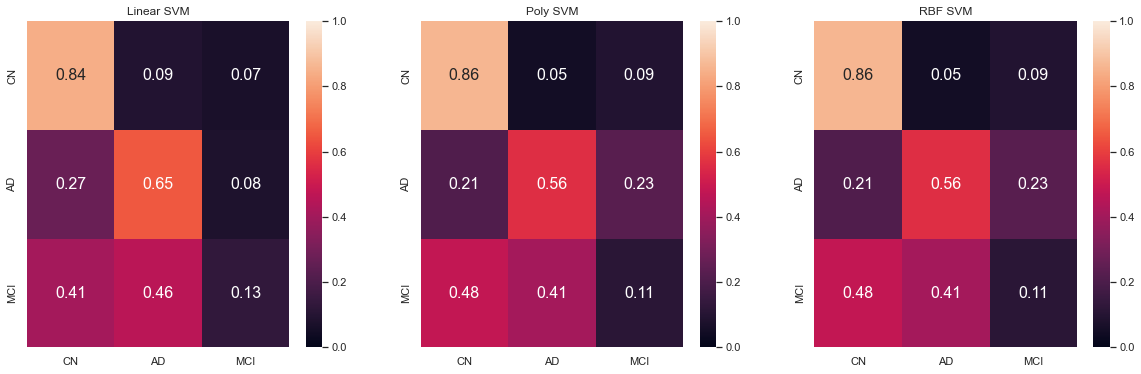
\includegraphics[width=\textwidth]{figures/Results/FAMD/FAMD_CM_with.png}
%     \caption[\en{FAMD SVM Confusion Matrices with scaling and balancing}]{\en{The Confusion Matrices for each class, per SVM kernel, for the FAMD transformed imaging and genetic data.}}
% \end{figure}

\begin{figure}[H]
    \centering
    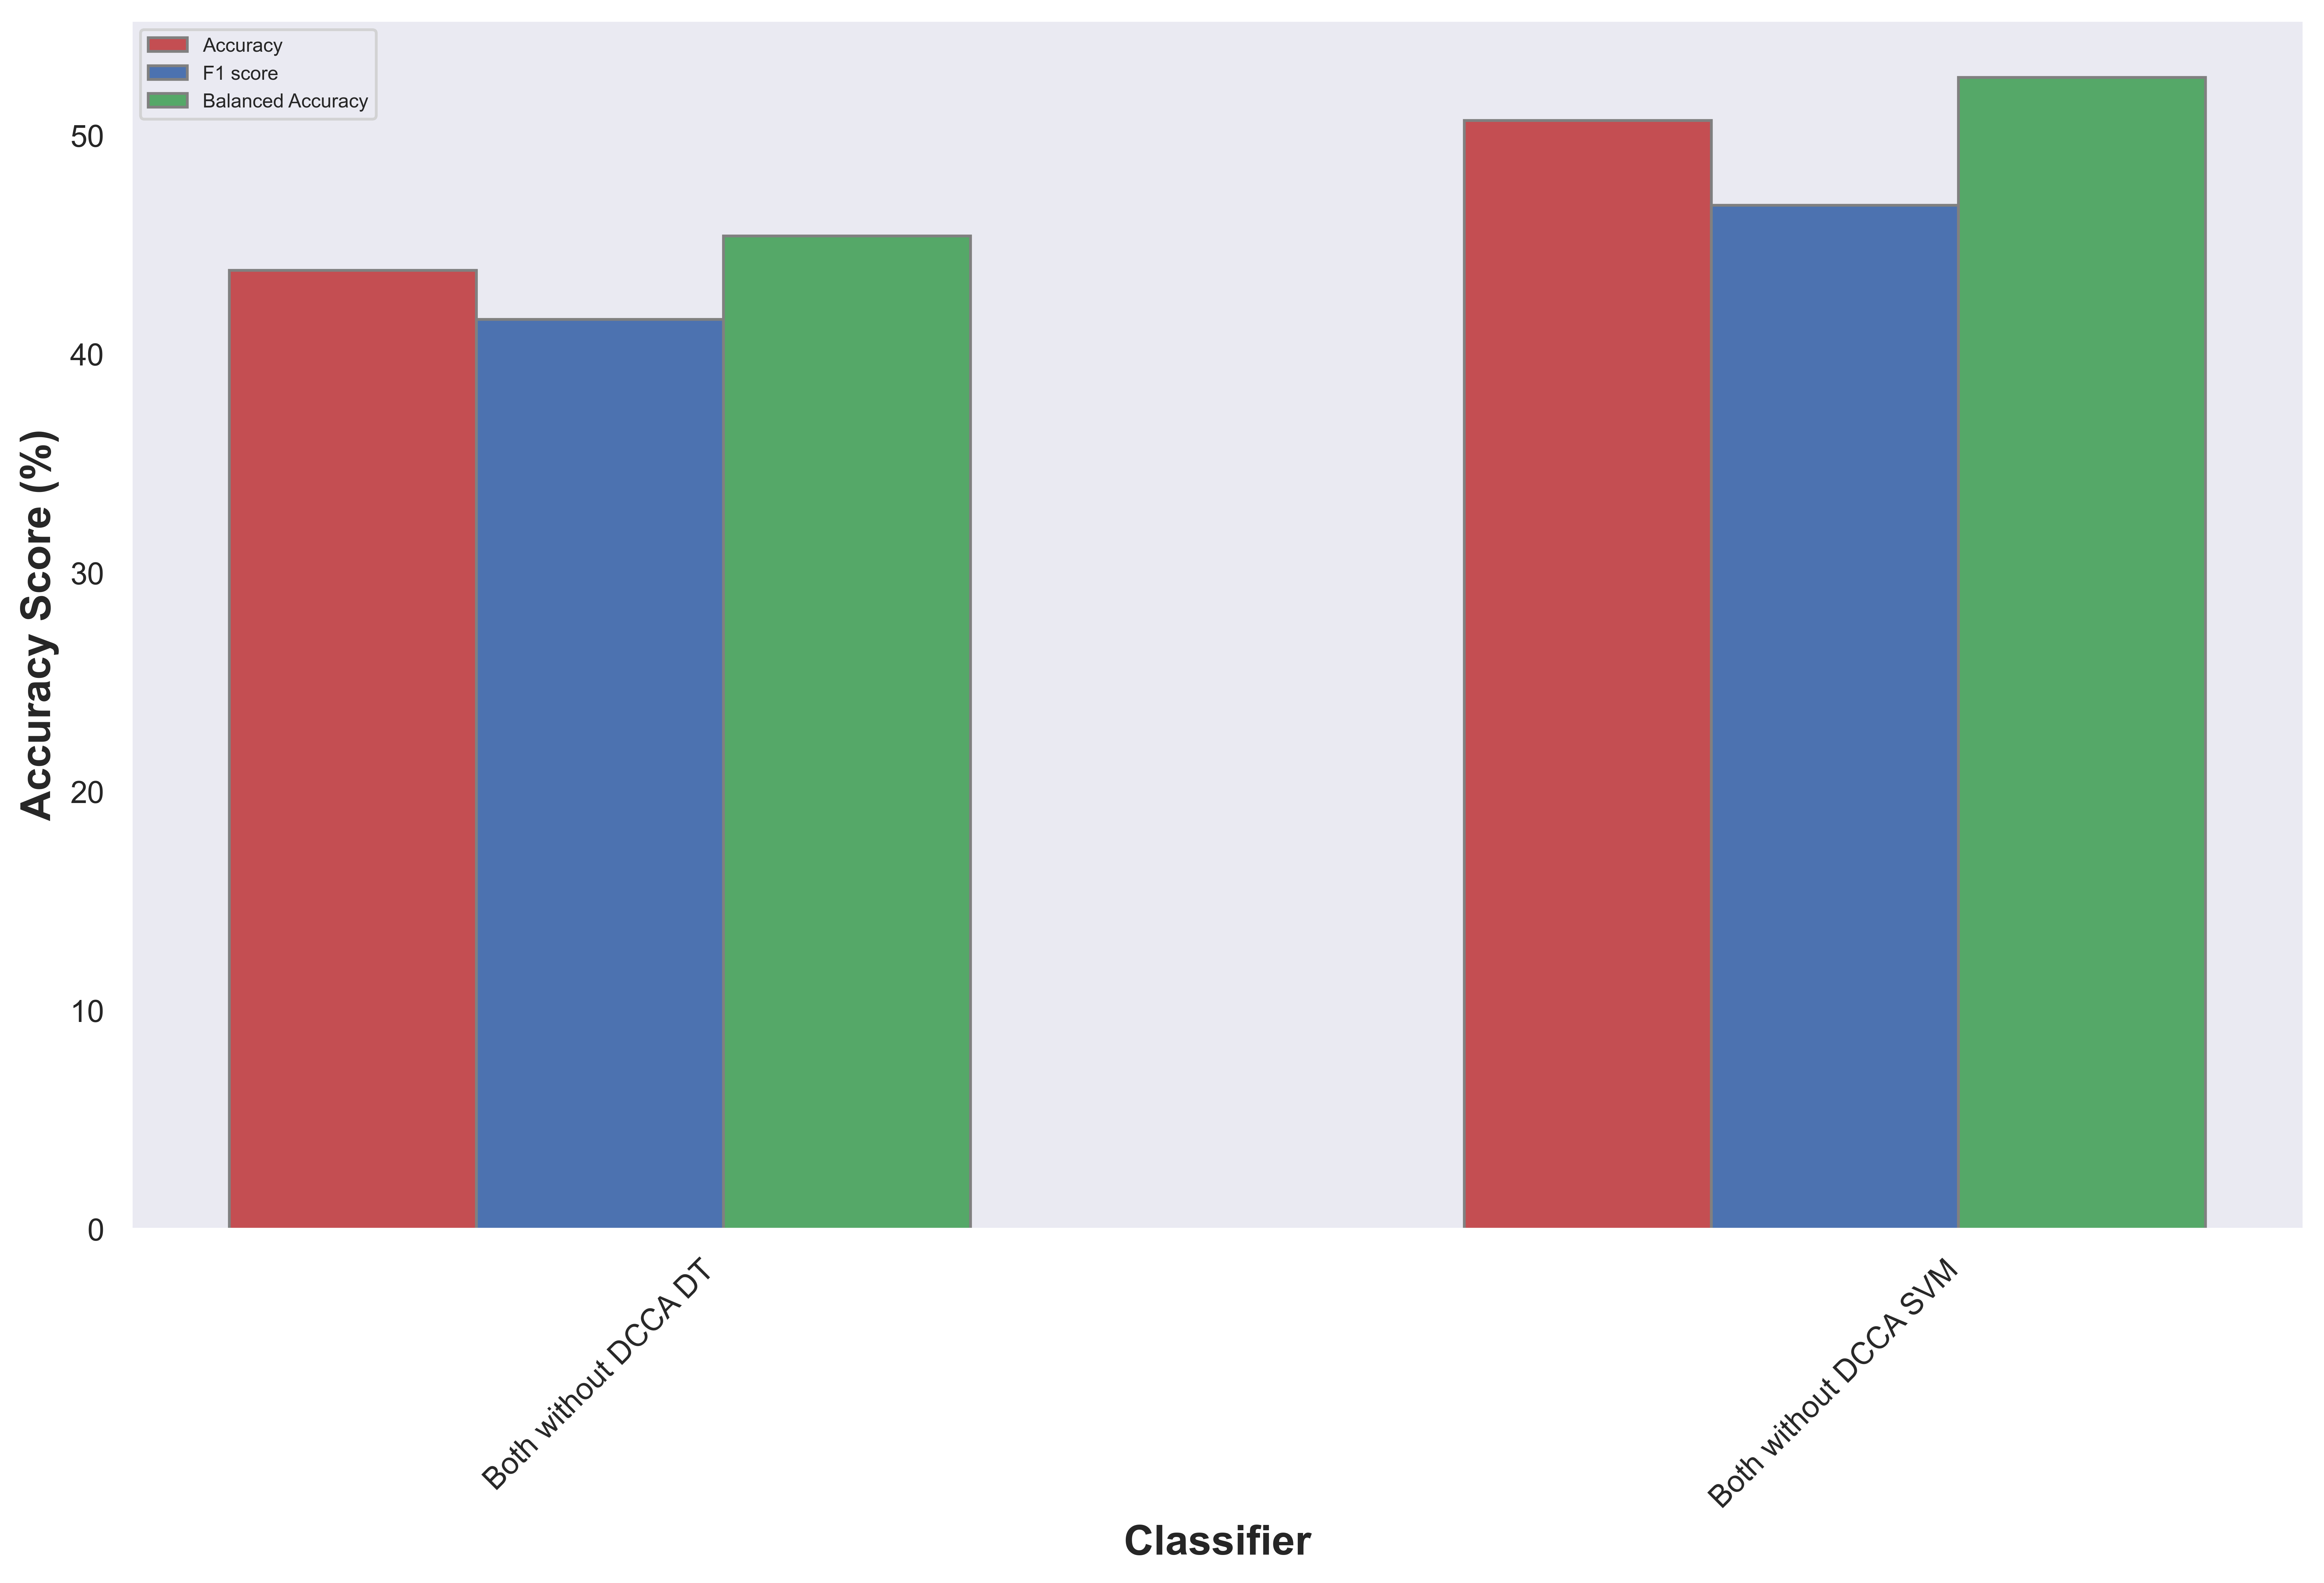
\includegraphics[width=\textwidth]{figures/Results/FAMD/Bagging_FAMD_with.png}
    \caption[\en{FAMD Bagging Classification metrics with scaling and balancing}]{\en{Classification metric using Bagging on the FAMD transformed imaging and genetic data.}}
\end{figure}

% \begin{figure}[H]
%     \centering
%     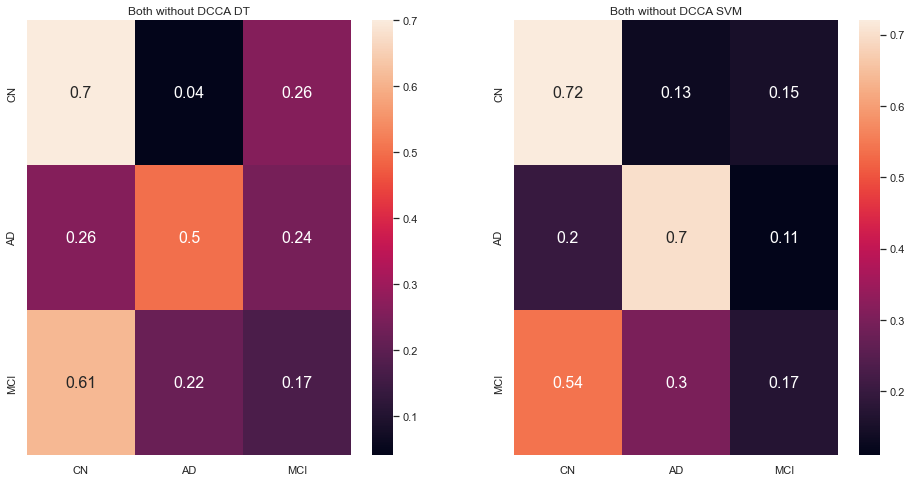
\includegraphics[width=\textwidth]{figures/Results/FAMD/Bagging_FAMD_CM_with.png}
%     \caption[\en{FAMD Bagging Confusion Matrices with scaling and balancing}]{\en{The Confusion Matrices for each class, with Bagging, for the FAMD transformed imaging and genetic data.}}
% \end{figure}

\begin{figure}[H]
    \centering
    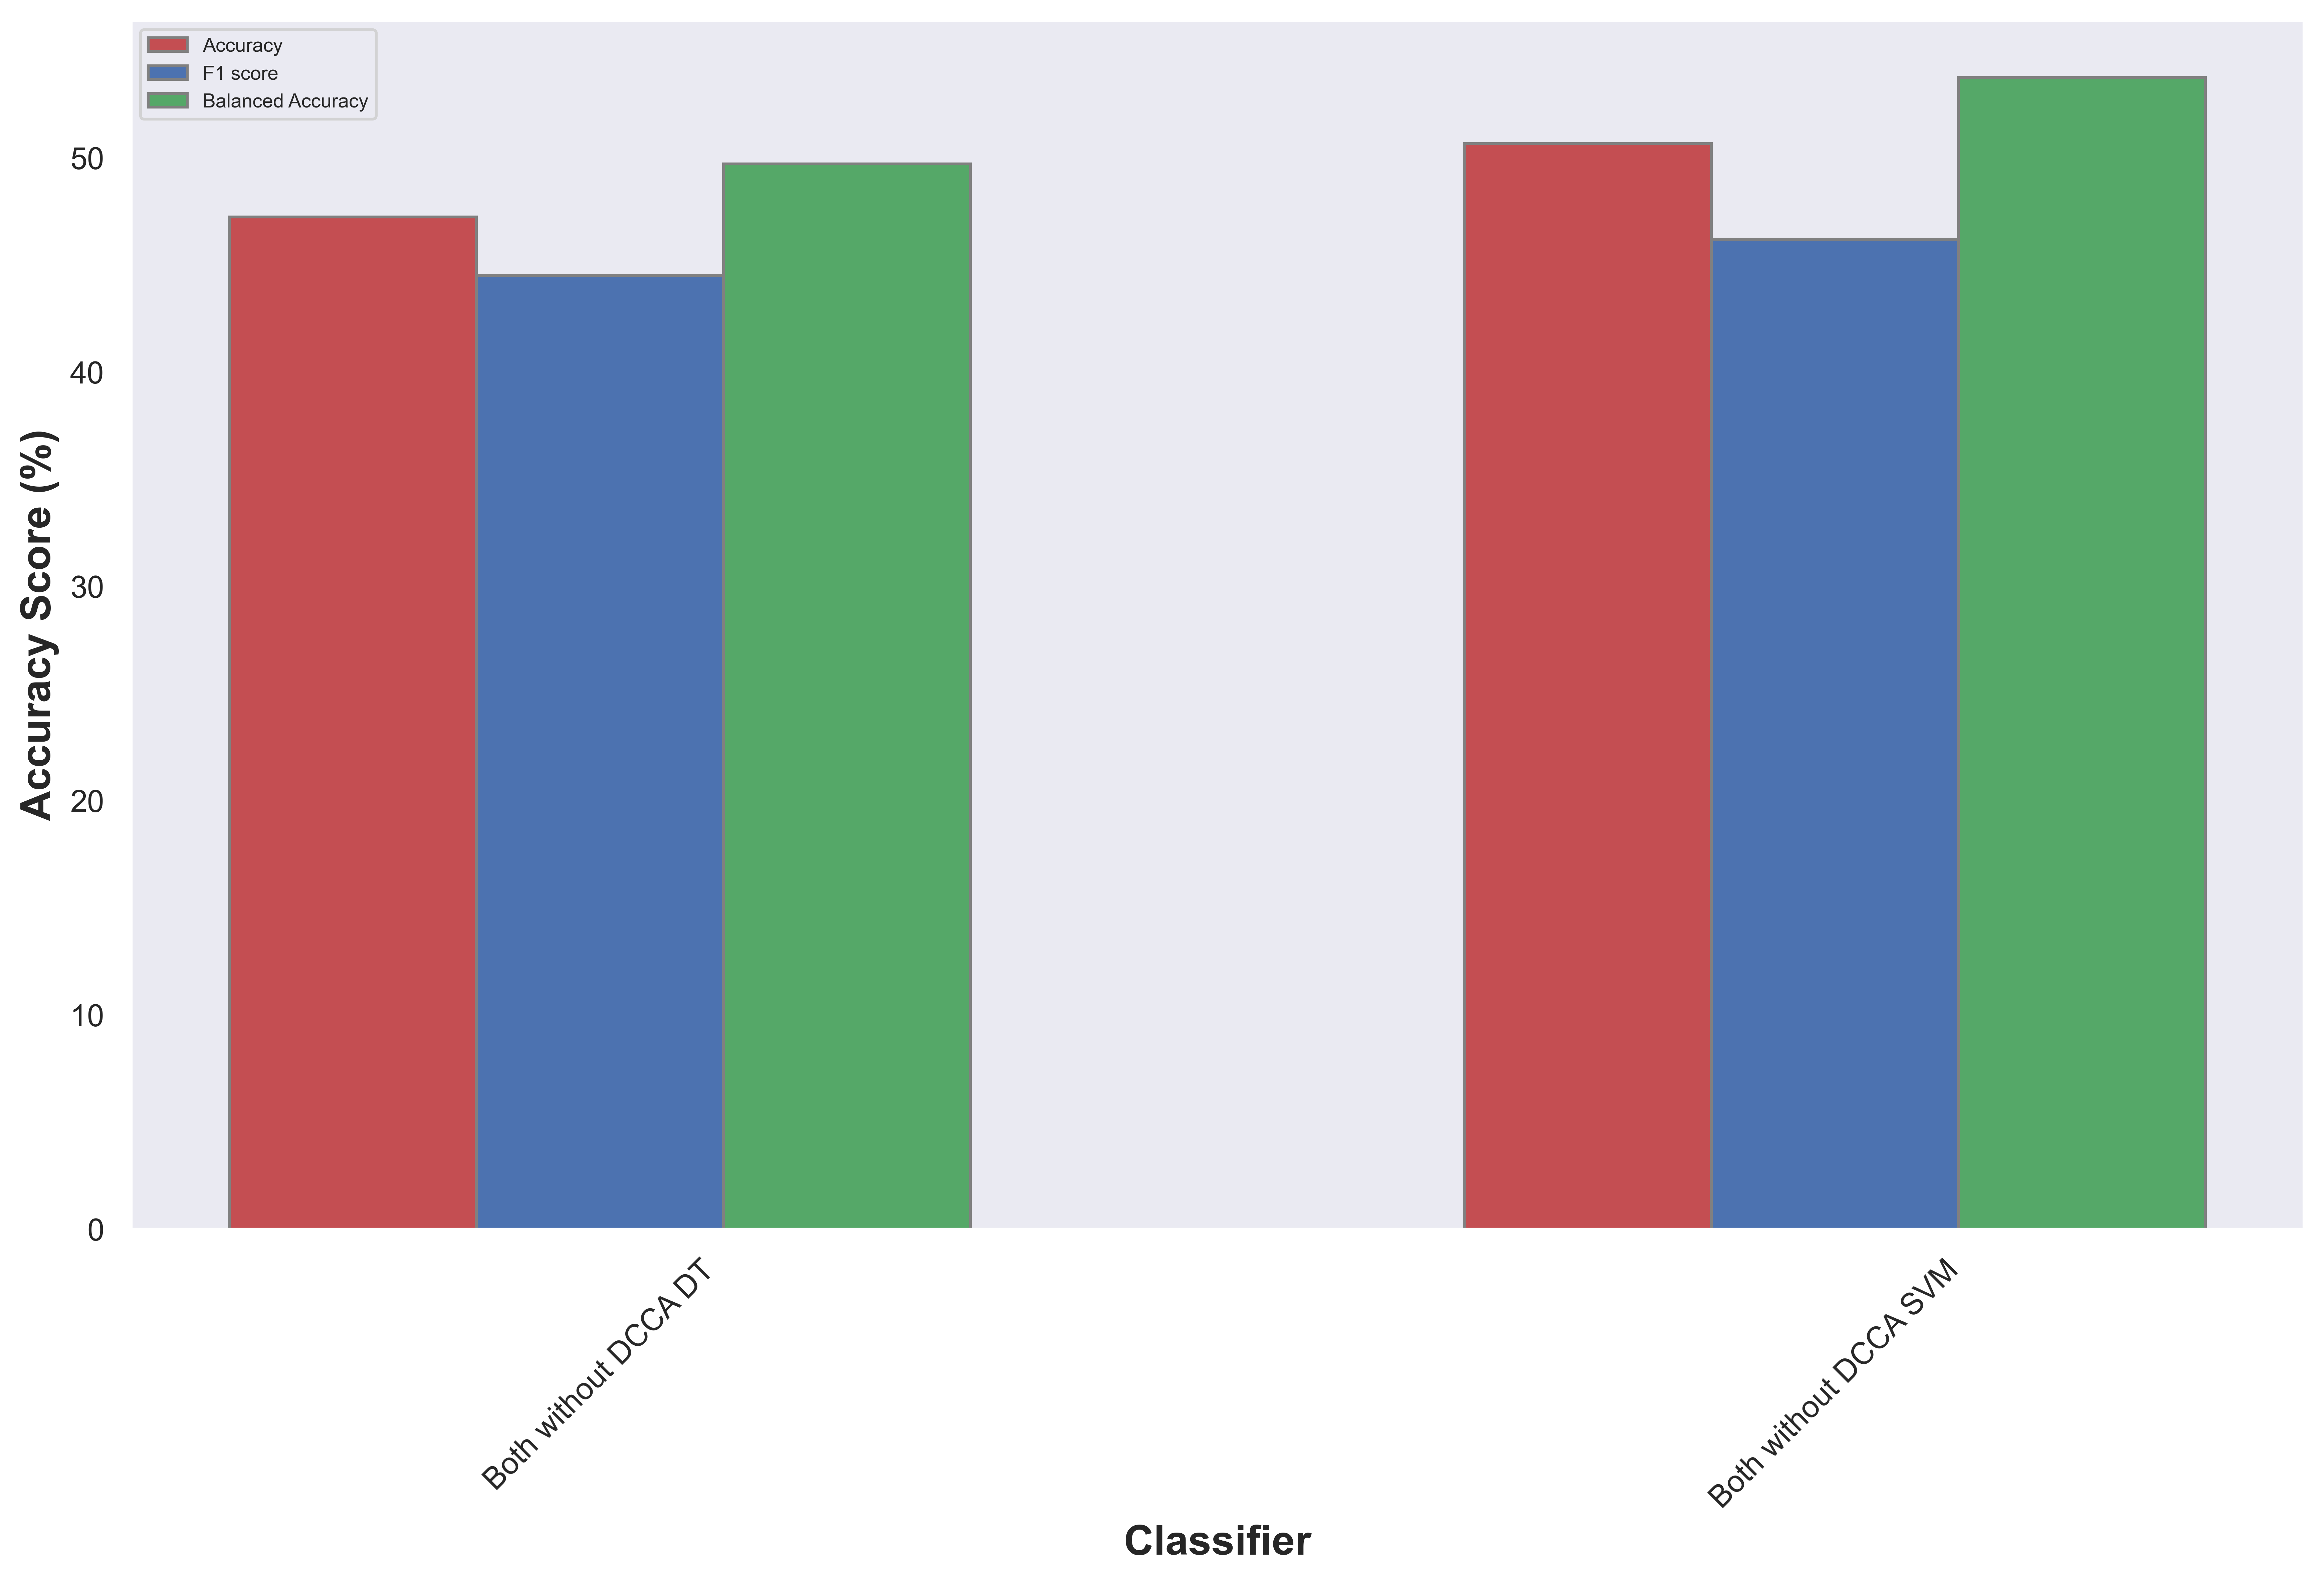
\includegraphics[width=\textwidth]{figures/Results/FAMD/AdaBoost_FAMD_with.png}
    \caption[\en{FAMD AdaBoost Classification metrics with scaling and balancing}]{\en{Classification metric using AdaBoost on the FAMD transformed imaging and genetic data.}}
\end{figure}

% \begin{figure}[H]
%     \centering
%     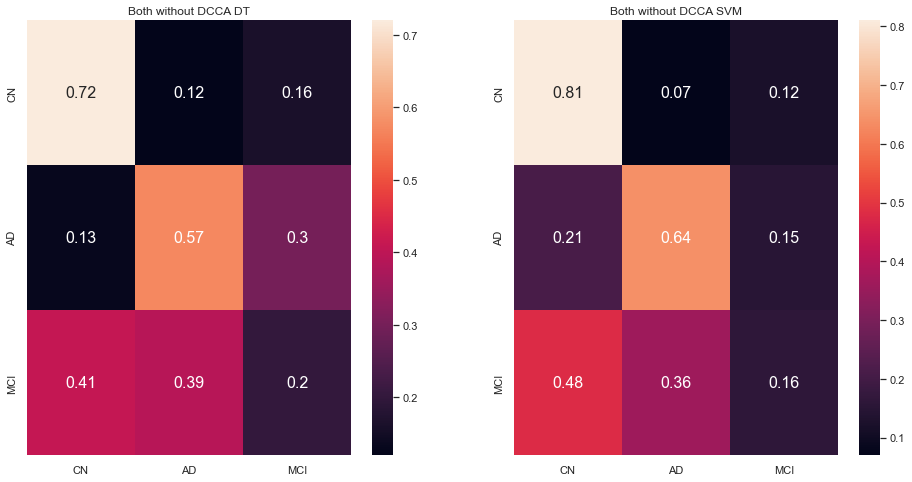
\includegraphics[width=\textwidth]{figures/Results/FAMD/AdaBoost_FAMD_CM_with.png}
%     \caption[\en{FAMD AdaBoost Confusion Matrices with scaling and balancing}]{\en{The Confusion Matrices for each class, with AdaBoost, for the FAMD transformed imaging and genetic data.}}
% \end{figure}

The following tables present the complete results for the FAMD transformed data, for each model, for each metric, for each view, and either with or without scaling and balancing. With green are highlighted the best values for each metric, depending on whether scaling and balancing were applied:

\begin{figure} [H]
    \centering
    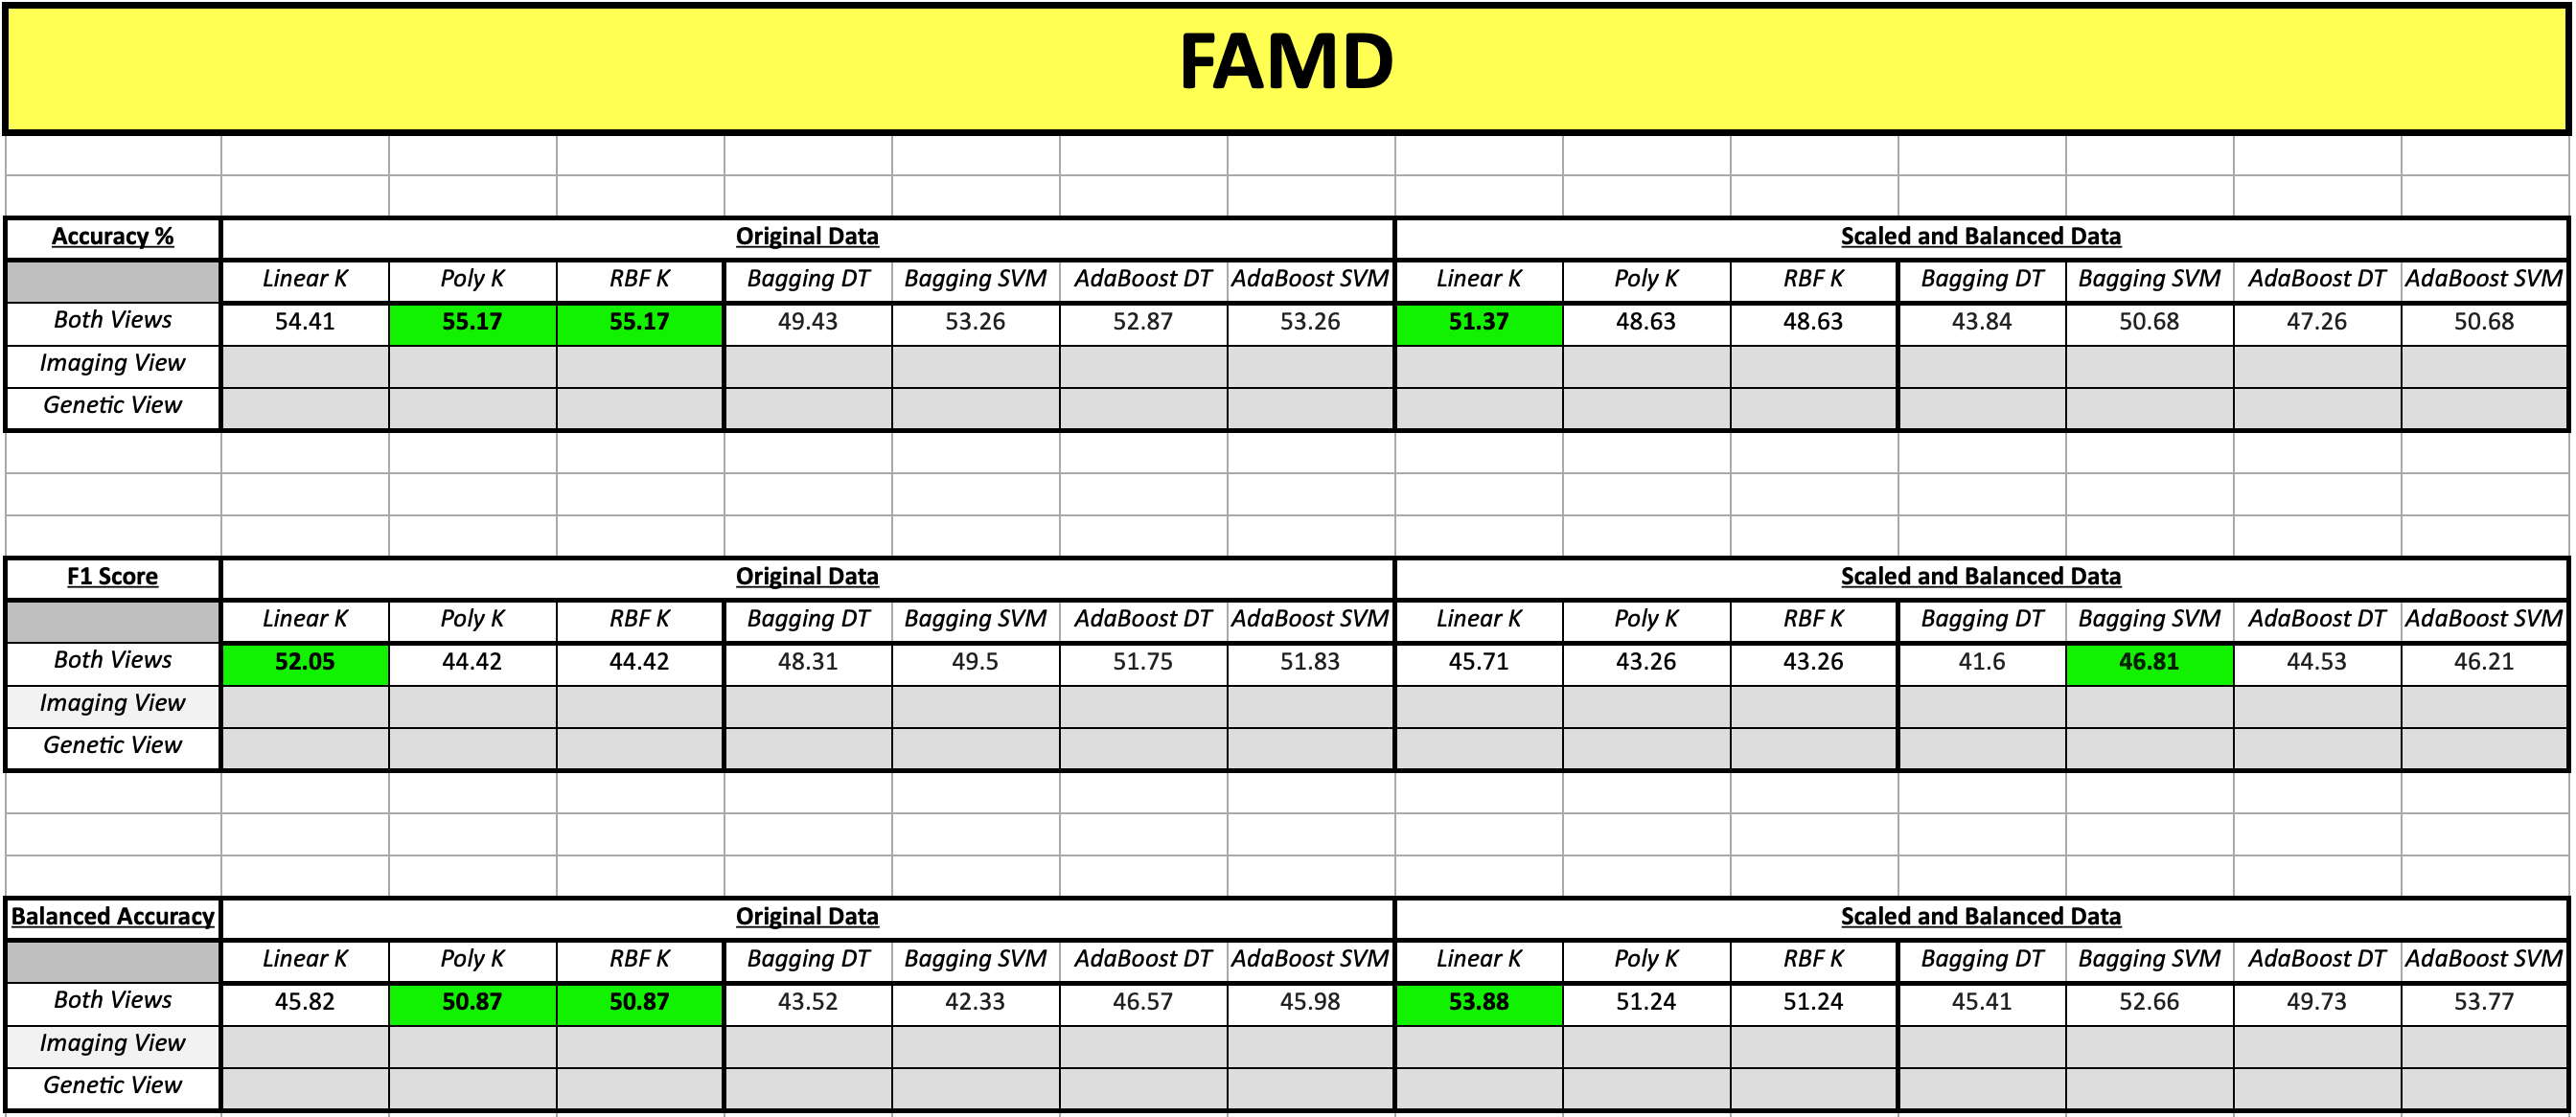
\includegraphics[width=\textwidth]{figures/Results/Analytical_Table_FAMD.png}
    \caption[\en{Analytical table of results for FAMD data classification}]{\en{For each model and classifier, the metric scores for FAMD transformed data classification are presented. Highlighted green are the best performing models, for each metric.}}
    \label{fig: Summary Table for classification scores for FAMD data}
\end{figure}
}